\documentclass[tikz]{standalone}
\usetikzlibrary{automata,positioning}
\begin{document}

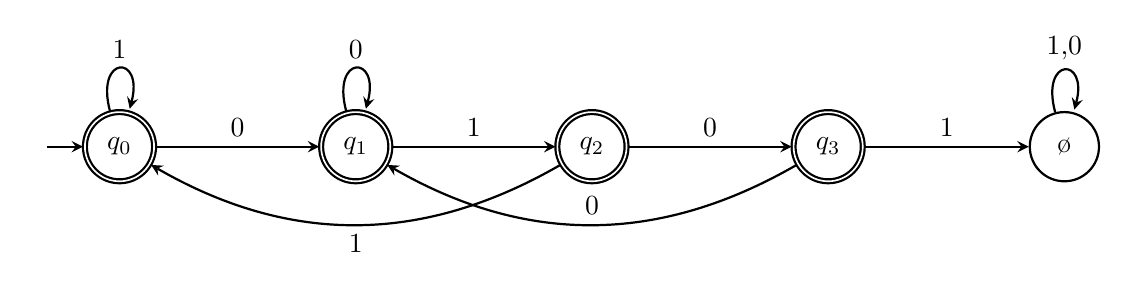
\begin{tikzpicture}[>=stealth,node distance=3cm,on grid,auto, thick, initial text=] 
  \node[state,initial,accepting] (q_0)   {$q_0$}; 
  \node[state,accepting]         (q_1) [right=3cm of q_0] {$q_1$};
  \node[state,accepting]         (q_2) [right= of q_1] {$q_2$};
  \node[state,accepting]         (q_3) [right=of q_2] {$q_3$};
  \node[state]         			 (q_4) [right=of q_3] {$\o$};

  \path[->]            (q_0) edge [left] node [above] {0} (q_1)
                             edge [loop above] node [above] {1} (q_0)
                       (q_1) edge [loop above] node {0} (q_0)
                             edge [left] node[above] {1} (q_2)
                       (q_2) edge [left] node[above] {0} (q_3)
                             edge [bend left] node {1} (q_0)
                       (q_3) edge [bend left] node[above] {0} (q_1)
                             edge [left] node [above] {1} (q_4)
                       (q_4) edge [loop above] node[above] {1,0} (q_4);
\end{tikzpicture}
\end{document}